\chapter{Eficiência Energética}
\section{Consumo de Energia}

\subsection{Consumo energético por habitante}

	De acordo com os dados coletados no Anuário Estatístico de Energia Elétrica de 2013, a média de consumo de uma residência no Distrito Federal, dos anos de 2008 à 2012, é de 217,72 kWh/mês, porém, esses dados não levam em consideração o tamanho da habitação ou a quantidade de moradores. Segundo o mesmo anuário, cada habitante gasta em média 2,1532 kWh/dia e em média 65kWh mensal\cite{2013Aneel}.

\subsection{Consumo médio de uma família para 4 pessoas}

	Fazendo um cálculo meramente estatístico, numa estimativa grosseira, supondo um mês com 30 dias e 4 habitantes com a média de consumo idênticas, obtemos que o consumo médio de energia de uma residência com 4 pessoas sendo de 258,384 kWh/mês. Ainda de acordo com esses valores, pode-se supor que essa média não leva em consideração a classe social da família, onde, a grosso modo, sabe-se que quanto maior a renda familiar, maior serão os seus gastos. Como os equipamentos de segurança e outros objetos mais específicos voltados a automação e outros equipamentos que fogem do padrão residencial não foram bem detalhados, faz-se uma estimativa, ainda embasado no consumo médio residencial brasileiro, de que a família consumirá uma média de 500 \nicefrac{\si{\kilo\watt\hour}}{mês}.

\subsection{Horários de maior consumo}

	Composta por 4 moradores, baseado na média nacional, o modelo familiar ainda segue o padrão histórico, no caso, um casal com filhos. Ressaltando que não foram levados em consideração o conceito de família encontrado na legislação, portanto atribui-se o conceito de casal como a união entre homem e mulher baseando-se apenas nos dados do \cite{IBGE} quanto aos tipos de família. Para justificativas de cálculos e média de consumo da família, é importante que se estabeleça sua rotina, bem como as faixas etária de cada habitante. Ainda com base nos dados sobre a média etária da população, de acordo com o censo demográfico, estabeleceu-se que o casal tenha entre 30 – 44 anos, e os filhos, um entre 15 – 29 anos e o outro entre 0 – 14 anos.

	Sendo que, o casal trabalha em horário comercial e os filhos estão em idade escolar, permanecendo todos fora da casa durante o dia e se reunindo em casa no período noturno, a partir das 18h. Obedecendo assim os horários de consumo energético médio do país, onde os horários de consumo e de pico se fixam a partir das 18h até as 23h nos dias uteis.

\subsection{Fontes consumidoras}

	Abaixo encontra-se a tabela dos eletrodomésticos comuns usados pela família, baseado nos eletrodomésticos de uso comum encontrado na média das famílias brasileiras segundo dados da \cite{2013Aneel}, bem como dados referentes a potência de cada equipamento (dado encontrado pelas especificações do fabricante em cada aparelho), a quantidade de cada equipamento presenta na casa, o uso em horas por dia e a quantidade de dias num mês em que se usa cada aparelho, por fim têm-se a última coluna onde calcula-se o consumo mensal de cada aparelho e no fim o resultado do consumo médio mensal da residência. Para o cálculo de consumo médio não se levou em consideração os equipamentos de segurança, bem como sensores e câmeras de monitoramento, se tratando apenas de valores hipotéticos e apenas para fins estatísticos.

\begin{table}[H]
\noindent\begin{tabular}{|c|c|c|c|c|c|}
\hline
\textbf{Eletrodoméstico} & \textbf{Qte} & \textbf{Potência [\si{\watt}]} & \textbf{Uso Diário [\si{\hour}]} & \textbf{Qte dias/mês} & \textbf{[\si{\kilo\watt\hour}] Mensal}\tabularnewline
\hline
\hline
Ar condicionado & 4 & 1400 & 1 & 10 & 56\tabularnewline
\hline
Aspirador de pó & 1 & 600 & 1 & 5 & 3\tabularnewline
\hline
Batedeira & 1 & 100 & 1 & 4 & 0,4\tabularnewline
\hline
Computador & 1 & 300 & 1 & 30 & 9\tabularnewline
\hline
Fero Elétrico & 1 & 1000 & 2 & 4 & 8\tabularnewline
\hline
Fogão (cooktop) & 1 & 3000 & 1 & 26 & 78\tabularnewline
\hline
Forno Elétrico & 1 & 1500 & 1 & 12 & 18\tabularnewline
\hline
Freezer\parnote{} & 1 & 300 & 10 & 30 & 90\tabularnewline
\hline
Geladeira\parnote{O tempo médio de 10 horas diárias para geladeira e freezer refere-se ao período em que o compressor fica ligado para manter o interior na temperatura desejada\label{compressor}} & 1 & 115 & 10 & 30 & 34,5\tabularnewline
\hline
Home Theatre & 1 & 150 & 2 & 4 & 1,2\tabularnewline
\hline
Lâmpadas & 30 & 6 & 5 & 20 & 18\tabularnewline
\hline
Lava-louças & 1 & 1500 & 1 & 4 & 6\tabularnewline
\hline
Liquidificador & 1 & 200 & 0,5 & 10 & 1\tabularnewline
\hline
Máquina de lavar & 1 & 1000 & 2 & 5 & 10\tabularnewline
\hline
Microondas & 1 & 2000 & 0,5 & 15 & 15\tabularnewline
\hline
Notebook & 4 & 65 & 2 & 26 & 13,52\tabularnewline
\hline
Secador & 1 & 1000 & 0,5 & 30 & 15\tabularnewline
\hline
Televisão & 3 & 90 & 2 & 30 & 16,2\tabularnewline
\hline
Vídeo game & 1 & 20 & 2 & 15 & 0,6\tabularnewline
\hline
\multicolumn{5}{|c|}{\textbf{Consumo total mensal [\si{\kilo\watt\hour}/mes]}} & 393,42\tabularnewline
\hline
\end{tabular}
\parnotes
\caption{Consumo mensal dos eletrodomésticos}
\label{consumo_eletrodomesticos}
\end{table}

Para cálculo do consumo mensal foi utilizado a seguinte expressão:

\begin{equation*}
	C_m = \sum \dfrac{P * Q_a * U_d * Q_d}{1000}
\end{equation*}

Onde $P$ é a potência, valor encontrado nas especificações de cada aparelho dado em watts [\si{\watt}]. $Q_a$ é a quantidade de aparelhos, o número referente à quantidade de um mesmo aparelho presente na casa, valor adimensional. $U_d$ é o uso diário, tempo estimado em que o equipamento consome energia elétrica da casa por dia, valor em horas [\si{\hour}]. $Q_d$ é a quantidade de dias, o número de dias em que o equipamento é usado ligado à rede elétrica no período de um mês, sendo considerado um mês com 30 dias, valor adimensional. E por fim, $C_m$ é o consumo mensal, é a soma do consumo de todos os aparelhos durante o mês, valor em quilowatt-hora \nicefrac{\si{\kilo\watt\hour}}{mês}.

\subsection{Valor da tarifa referente à CEB}
	
	De acordo com a ANEEL, a CEB homologou uma tarifa de 0,43676 reais por quilowatt-hora (\nicefrac{R\$}{\si{\kilo\watt\hour}}).
Valores na tabela abaixo, disponibilizada pela ANEEL.

\begin{table}[H]
\centering
\begin{tabular}{|l|c|}
\hline 
\multicolumn{2}{|l|}{Empresa: CEB-DIS - CEB Distribuição S.A.}\tabularnewline
\hline 
\multicolumn{2}{|l|}{Vigência da Tarifa de 26/08/2015 a 25/08/2016}\tabularnewline
\hline 
\multicolumn{2}{|l|}{Resolução Homologatória N\textsuperscript{o}1937 Publicada em 26/08/2015\cite{2015ResolucaoAneel}}\tabularnewline
\hline 
\multicolumn{2}{|l|}{Variação percentual em relação ao período anterior: 18,66\%}\tabularnewline
\hline 
\hline 
Descrição & R\$/kWh\parnote{Os Valores constantes da resolução homologatória referida são expressos
em \nicefrac{R\$}{\si{\kilo\watt\hour}}}\tabularnewline
\hline 
B1 - Residencial & 0,43676\tabularnewline
\hline 
B1 - Residencial Baixa Renda & \tabularnewline
\hline 
Consumo mensal inferior ou igual a 30 kWh & 0,15060\tabularnewline
\hline 
Consumo mensal superior a 30 kWh e inferior ou igual a 100 kWh & 0,25817\tabularnewline
\hline 
Consumo mensal superior a 100 kWh e inferior ou igual a 220 kWh & 0,38725\tabularnewline
\hline 
Consumo mensal superior a 220 kWh & 0,43028\tabularnewline
\hline 
\end{tabular}
\parnotes
\caption{Valores das tarifas energéticas disponibilizada pela ANEEL}
\end{table}

Os valores acima se referem às tarifas homologadas pela ANEEL, expressas na unidade \nicefrac{R\$}{\si{\kilo\watt\hour}} (reais por quilowatt-hora) e não contemplam tributos e outros elementos que fazem parte de sua conta de luz, tais como: ICMS, Taxa de Iluminação Pública e Encargo de Capacidade Emergencial, cuja cobrança foi encerrada em 22 de dezembro de 2005.

\subsection{Valores monetários do consumo família}

	Uma família de 4 pessoas consumirá em média 500 kWh/mês. Caso a casa usasse a energia totalmente da rede elétrica disponibilizada pelo Distrito Federal (energia da concessionária de luz – CEB) o valor pago por mês seria em média R\$ 218,38.

	$V_{alor mensal}\ =\  \nicefrac{R\$}{\si{\kilo\watt\hour}}\times\nicefrac{\si{\kilo\watt\hour}}{mês}\ =\ 0,43676\times500\ =\ R\$ 218,38$


\subsection{Valores Reduzidos}
	
	A Agência Nacional de Energia Elétrica (Aneel) divulgou a Resolução Normativa no 482, em que estabelece os parâmetros regulatórios para a microgeração (até $100 \si{\kilo\watt}$) e a minigeração (entre $100 \si{\kilo\watt}$ e $1\si{\mega\watt}$) de energia elétrica a partir de sistemas particulares conectados à rede de distribuição. Ela viabiliza a geração distribuída de pequeno porte no Brasil.

	Nessa resolução, diversos parâmetros decisivos para o desenvolvimento desse novo mecanismo de produção energética foram estabelecidos, permitindo a produção de  energia a partir de unidades consumidoras e a disponibilização do excedente energético para a rede pública por meio de um simples sistema de compensação.

	O sistema de compensação, conhecido internacionalmente como net metering, irá adicionar à conta do consumidor toda a energia que ele utilizar do sistema público e irá subtrair dela toda a energia que ele injetar na rede, proveniente da geração a partir de sistemas fotovoltaicos e eólicos, como é o caso da casa sustentável.

	Caso a residência utilize mais energia do que produziu, irá pagar o equivalente de quilowatt-hora utilizado referente às tarifas às quais o estabelecimento corresponde. Por outro lado, caso a residência produza mais energia elétrica do que consuma, pagará apenas uma taxa fixa estabelecida pela concessionária e usufruirá de créditos válidos por 36 meses, que poderão ser abatidos as próximas faturas do próprio imóvel ou de outro imóvel definido pelo proprietário.

	De acordo com essa legislação por ser usado um sistema trifásico uma taxa mínima de $100 \si{\kilo\watt}$ deve ser paga mensalmente, o que acarretará em um custo mensal de R\$43,67.

	As informações estarão na fatura do consumidor, a fim de que ele saiba o saldo de energia e tenha o controle sobre a sua fatura.

\section{Fontes de Energia}

\subsection{O que são fontes renováveis?}

	As fontes de energia renováveis, são aquelas em que a sua utilização e uso é renovável e pode-se manter e ser aproveitado ao longo do tempo sem possibilidade de esgotamento dessa mesma fonte, exemplos deste tipo de fonte são a energia eólica e solar\cite{2007RevUSP}

\subsection{Benefícios de energia renovável}

	As energias renováveis não poluem o ambiente e tem caráter inteiramente sustentável. No geral, causam um pequeno impacto (poluição, desmatamento) ao meio ambiente. Portanto, são excelentes alternativas ao sistema energético tradicional, principalmente numa situação de luta contra a poluição atmosférica e o aquecimento global.

\subsection{Fontes utilizadas -- Justificativa}
\subsubsection{Solar}

	A Alemanha teve em 2014, cerca de 6,8\% da energia elétrica consumida produzida por placas fotovoltaicas (WIRTH, 2015). E este país possui um potencial solar inferior ao brasileiro. Contudo, o Governo investiu de forma eficaz para que ela competisse com as outras fontes presentes no país como a energia nuclear. Isso ocorreu, principalmente, devido ao acidente nuclear em Fukushima no Japão em 2011. Os países que dependiam da energia nuclear, como a Alemanha, viram nas fontes renováveis uma possível solução.

	A tabela \ref{irradiacao_media_anual} compara o potencial solar entre Brasil e Alemanha. Como pode ser observado na tabela, o potencial brasileiro é consideravelmente superior ao alemão, mas a participação da energia solar na matriz elétrica nacional é bem inferior à alemã. França e Espanha também possuem menor potencial mas também possuem uma maior porcentagem da matriz elétrica composta pela energia fotovoltaica. Isso se deve, pelo falta subsídio por parte do Governo para reduzir o custos que são altos para o consumidor.

\begin{table}[H]
\centering
\begin{tabular}{|c|c|c|c|c|}
\hline 
\textbf{Tópicos} & \textbf{Alemanha} & \textbf{Brasil} & \textbf{França} & \textbf{Espanha}\tabularnewline
\hline
\hline 
\textbf{Irradiação Global} & \multirow{2}{*}{900 e 1.250} & \multirow{2}{*}{1.200 e 2.400} & \multirow{2}{*}{900 e 1.650} & \multirow{2}{*}{1.200 e 1850}\tabularnewline
\textbf{Horizontal\nicefrac{\nicefrac{\si{\kilo\watt\hour}}{\si{\meter}$^2$}}{ano}} &  &  &  & \tabularnewline
\hline 
\end{tabular}
\caption{Irradiação média anual, EPE - Análise da Inserção da Geração Solar na Matriz Elétrica Brasileira}
\label{irradiacao_media_anual}
\end{table}

Mesmos com os custos altos, o investimento é pago com um certo período de tempo. A energia solar foi escolhida para o projeto em Brasília devido aos estudos feitos em relação a radiação global anual na região. A figura 1 mostra que a média anual de radiação incidente nesta área é de aproximadamente 20\nicefrac{\si{\mega\joule}}{\si{\meter$^2$}} dia.

\begin{figure}[H]
\centering
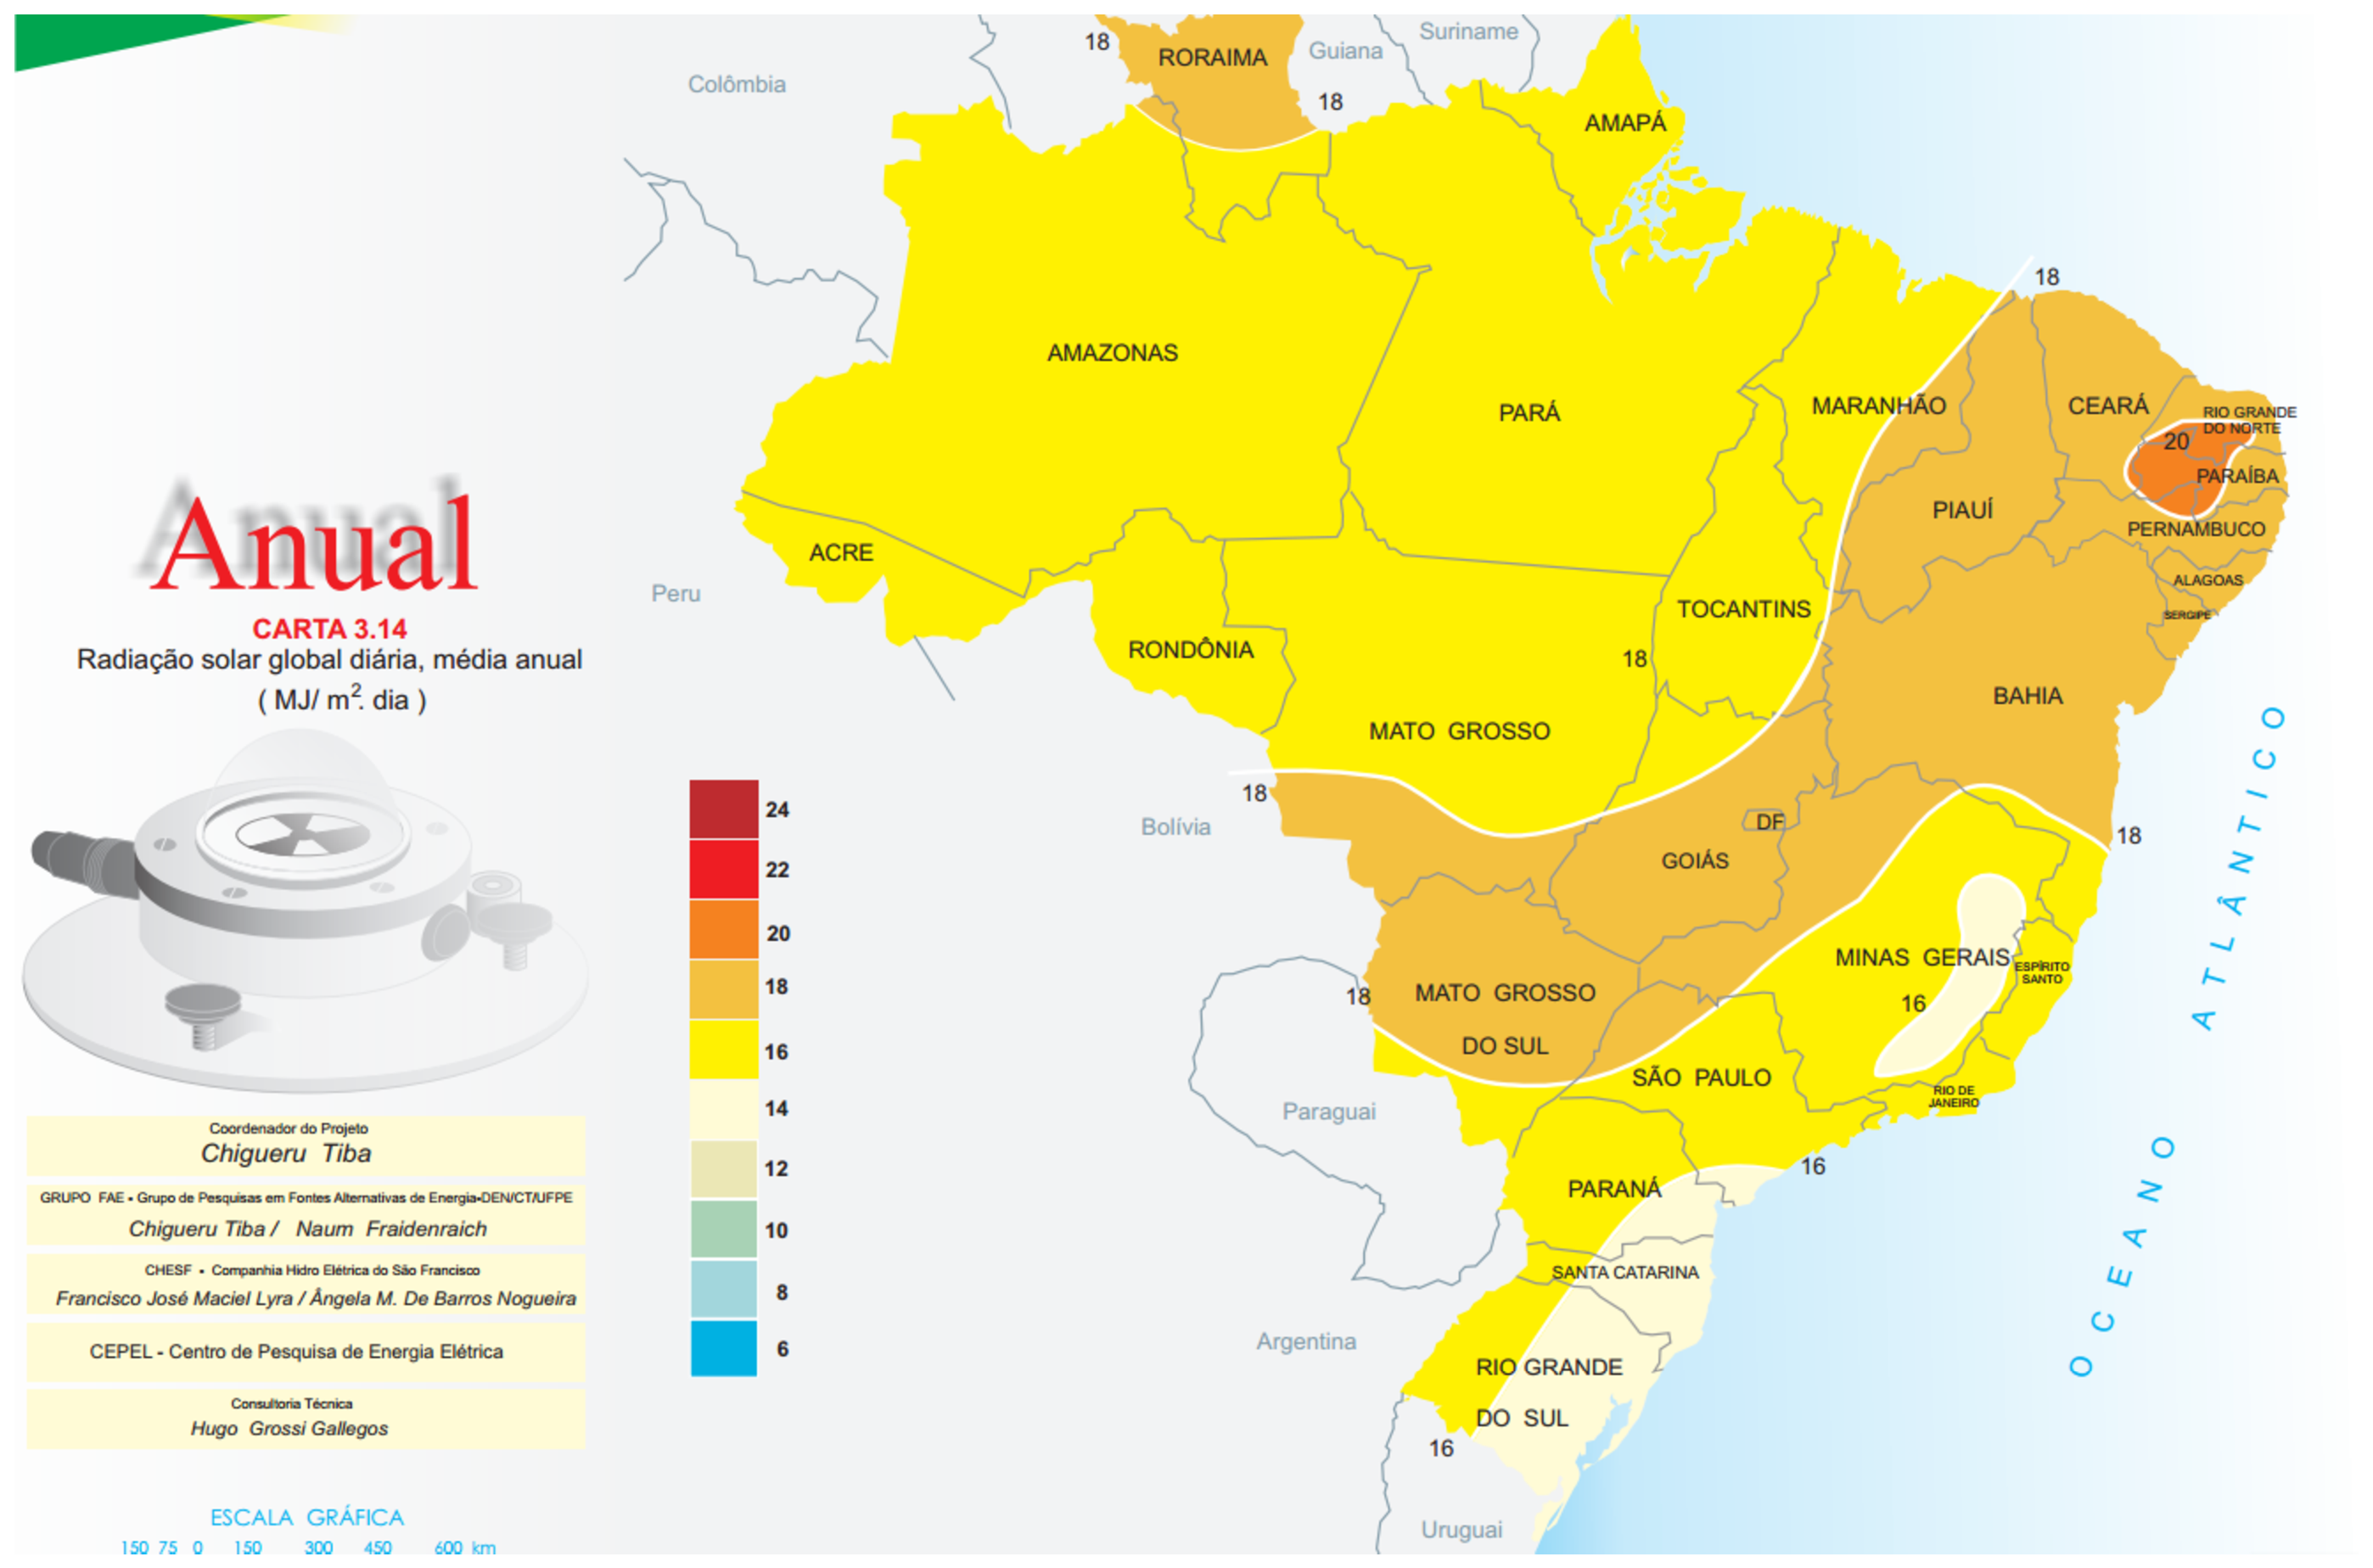
\includegraphics[width=.7\linewidth,keepaspectratio,angle=0]{figuras/radiacao_solar.eps}
\caption{Radiação solar global diária, média anual.}
\end{figure}

	A irradiação aproveitada pela fonte fotovoltaica é Irradiação Global Horizontal (GHI), onde quantifica em uma superfície plana a quantidade de radiação recebida. Esta radiação é divida em Irradiação Difusa Horizontal (DIF) e Irradiação Normal Direta (DNI). A DIF é uma quantidade dispersa por reflexões em elementos na atmosfera como poeira e as nuvens. A DNI é a irradiação que não sofre reflexões, atingindo o solo diretamente. (2)

	A determinação da posição dos painéis solares depende da variação da posição da Terra em relação ao Sol ao longo do ano, ao norte (azimute) e ao plano horizontal. Esta orientação otimiza aproveitamento solar de painéis fixos. Brasília está localizada no hemisfério Sul, logo os painéis deverão estar voltados para o norte “verdadeiro” e a inclinação de acordo com o plano horizontal. Esta inclinação pode ser de acordo com as estações do ano ou com a produção media durante o ano. A escolha deverá ser feita a fim de maximizar a produção.(2)

	Os elementos semicondutores fotossensíveis das placas fotovoltaicas fazem a conversão da  radiação solar em diferença de potencial nos terminais de junção P-N2, que é a junção metalúrgica de dois cristais de natureza P e N, de acordo com sua composição atômica. A corrente contínua é resultante da ligação elétrica desses terminais. (2)

	Segundo Fadigas\cite{14}, a luz solar irá excitar a junção P-N e os fótons da luz irão se chocar com os elétrons da estrutura do silício. Desta forma, eles irão fornecer energia e transformara-os em condutores, criando um campo elétrico, no qual os elétrons fluem da camada P para a N, através de um condutor externo, gerando corrente elétrica (figura \ref{celula_fotovoltaica}).

\begin{figure}[H]
\centering
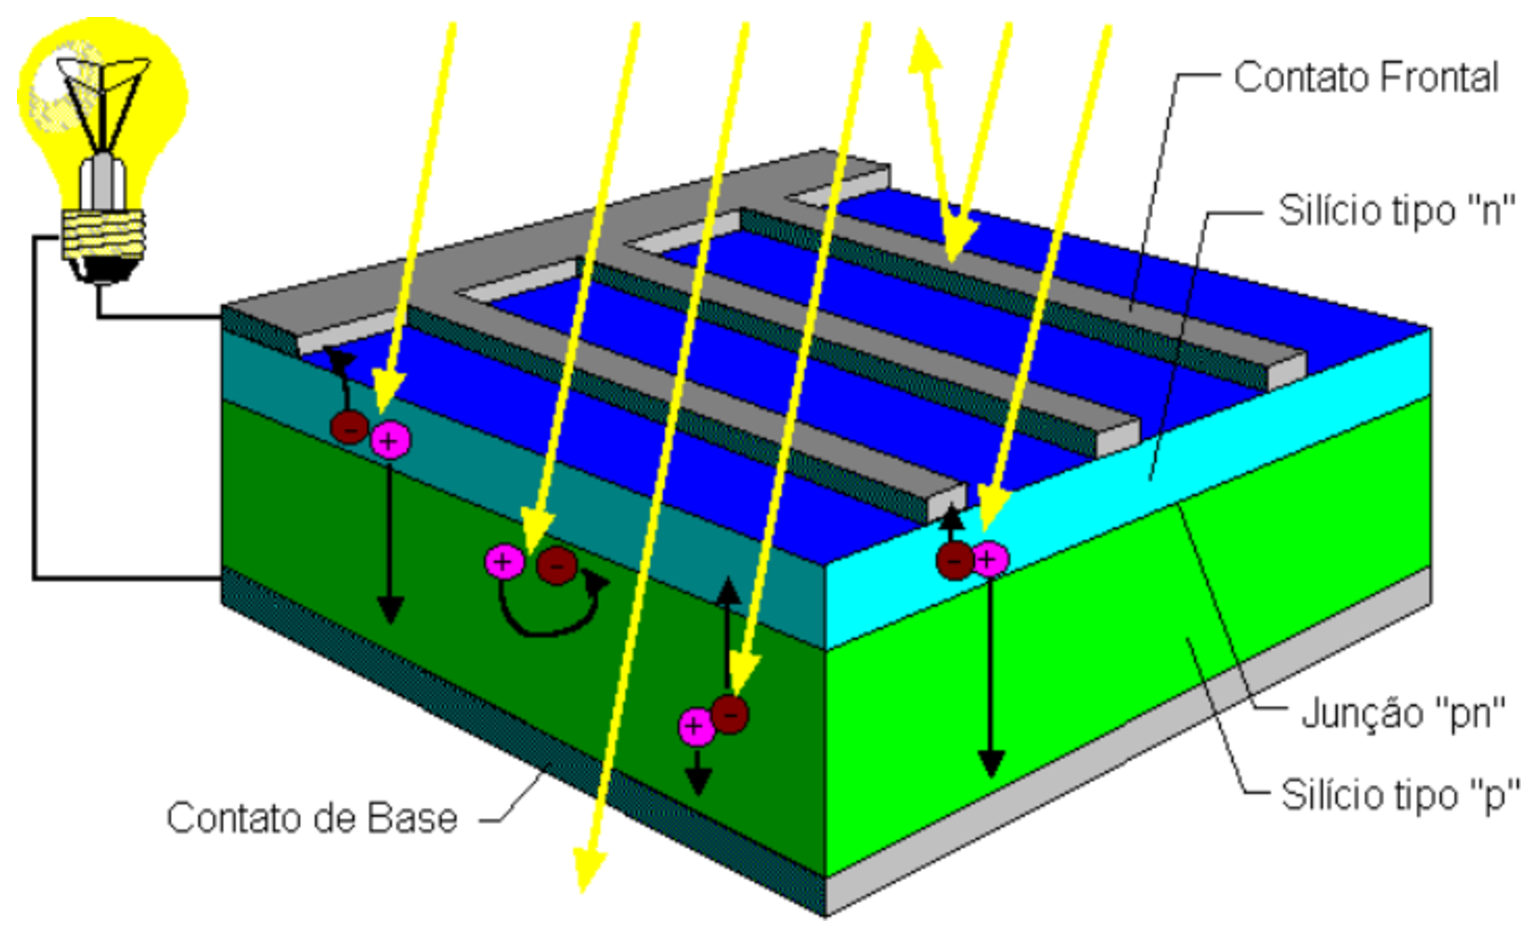
\includegraphics[width=.7\linewidth,keepaspectratio,angle=0]{figuras/celula_fotovoltaica.eps}
\caption{Célula fotovoltaica (corte transversal)\cite{1999CRESESBCEPEL}.}
\label{celula_fotovoltaica}
\end{figure}

	A condição de referência de eficiência do painel é a Standard Test Conditions – STC, que estabelece a relação da potência máxima de saída pela área da célula em $\si{\meter}^{2}$ e o padrão é $1000\nicefrac{\si{\watt}}{\si{\meter}^{2}}$, a $25^{o}C$. (2)

	A temperature ambiente de operação e a intensidade da irradiação solar incidente sobre a célula são os principais fatores que interferem na eficiência da conversão. 

	De acordo com a Resolução Normativa 482/2012 da ANEEL, o sistema fotovoltaico da casa será uma minigeração distribuída pois a potência instalada será superior a 100 kW e inferior a 1 MW e estará conectada à rede de distribuição. O consumidor não poderá vender sua energia para a distribuidora, ela entrará no sistema de compensação de energia elétrica. A compensação de energia  funcionará da seguinte forma: o sistema de distribuição receberá a energia ativa da unidade consumidora e essa energia será cedida a título de empréstimo gratuito para a distribuidora. A unidade consumidora terá 36 meses para consumir esse crédito em quantidade de energia ativa. (4)

\subsubsection{Eólica}

	O vento é o movimento horizontal e paralelo à superfície do planeta de parcelas de ar nas atmosferas planetárias. O vento é responsável pelo transporte de umidade e de energia na atmosfera como agente meteorológico. Já sua energia provoca grande destruição como furações e tornados. Porém, ele pode ser aplicado como uma fonte alternativa de energia, transformando energia cinética em eletricidade. (5)

	A energia cinética que está contida no vento é convertida em energia mecânica pelo giro das pás do rotor das turbinas eólicas. E depois é transformada em energia elétrica pelo gerador. A potência $p$ do vento e a velocidade u através de uma área A (área das hélices que interceptam o vento) é dada por:

$p\ =\ \cfrac{1}{2}\rho A u^{3}$

no qual $\rho$ é a densidade do ar. A máxima potência de uma turbina eólica é 59\%, mas ao  somar as perdas mecânicas, a potência total do vento utilizável reduz para 42\%.(5)

	O potencial eólico brasileiro também consideravelmente grande em comparação com vários outros países. Como pode ser visto na figura \ref{potencial_eolico}, o Brasil é capaz de produzir $272,2 \si{\tera\watt\hour}$ por ano. Contudo, o potencial da região Centro-Oeste é o menor dentre as 5 regiões brasileiras, com $5,4\si{\tera\watt\hour}$ por ano. O segundo menor que é a região Norte tem a capacidade produzir $26,4\si{\tera\watt\hour}$ por ano. 


\begin{figure}[H]
\centering
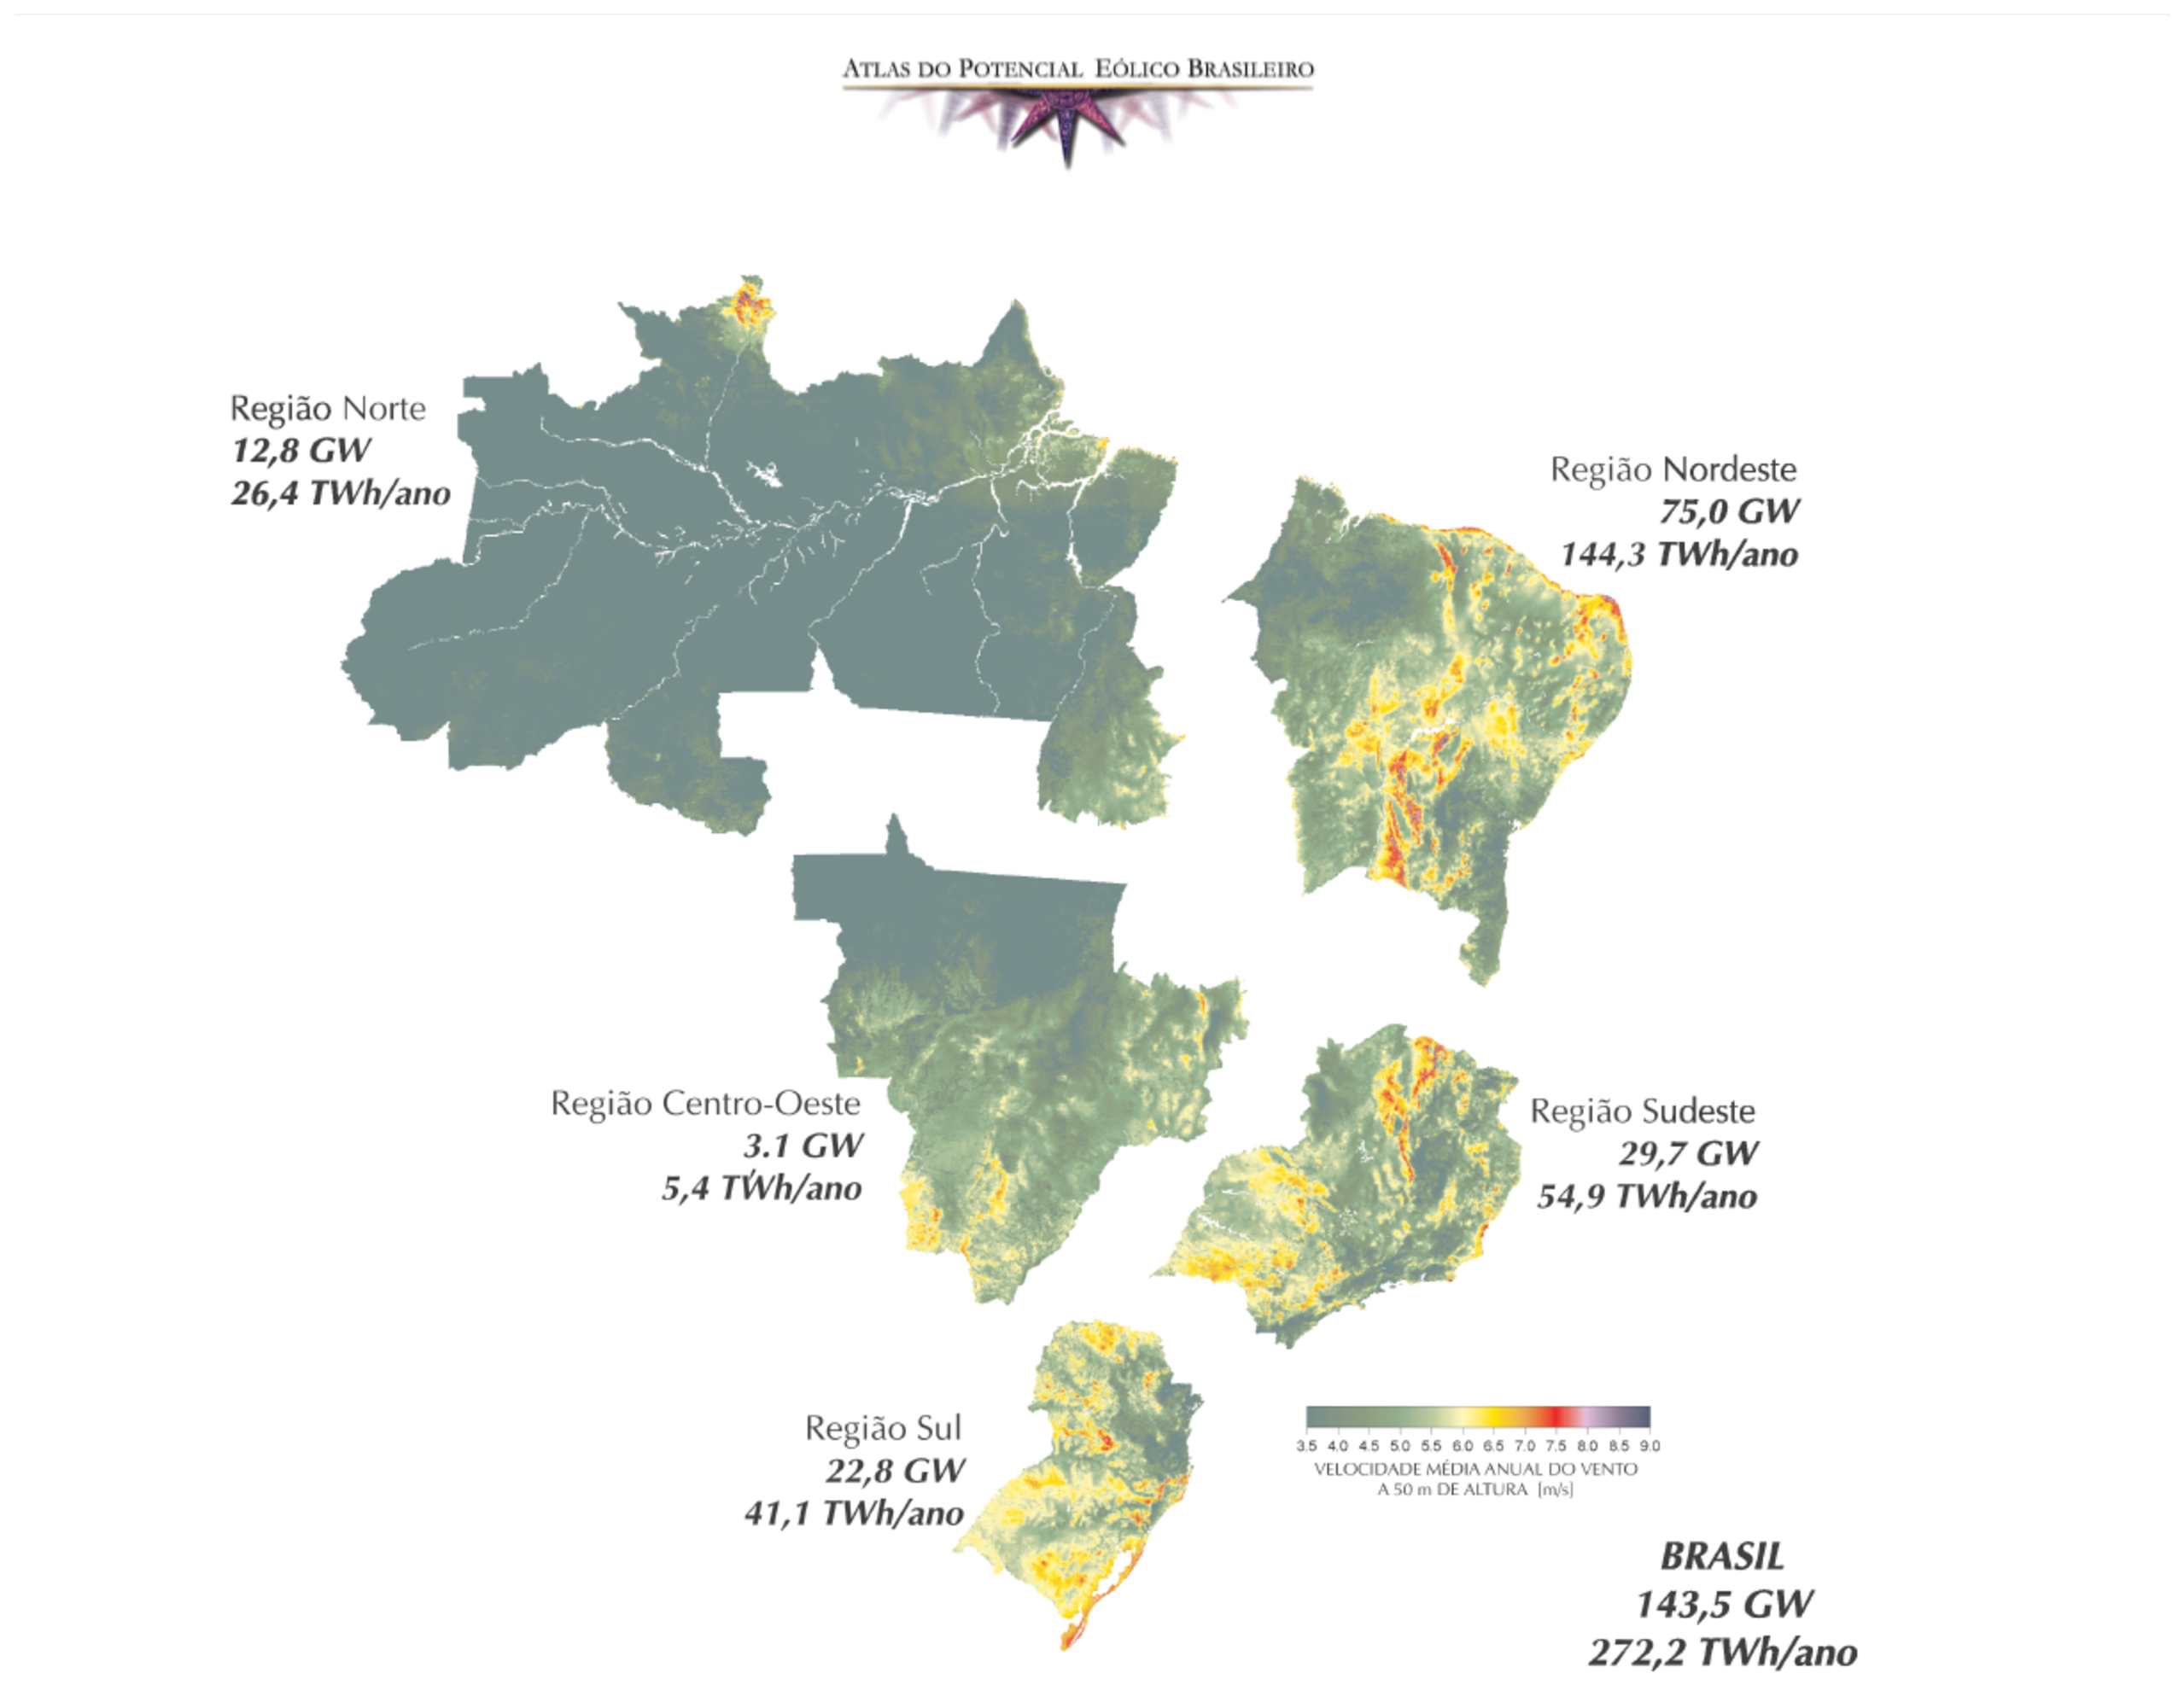
\includegraphics[width=.7\linewidth,keepaspectratio,angle=0]{figuras/potencial_eolico.eps}
\caption{Potencial eólico para vento médio anual igual ou superior a $7\nicefrac{\si{\meter}}{\si{\second}}$\parnote.}
\label{potencial_eolico}
\end{figure}

	A velocidade média anual do vento no Distrito Federal é 3,5m/s (Figura 4). Essa velocidade é suficiente para produzir uma pequena quantidade de energia. A fim de aproveitar essa energia e de solucionar outro problema, a energia eólica também será utilizada no projeto da casa. De acordo com Cormane (2015, por questão de segurança, quando houver falta de energia elétrica por parte da distribuidora, o sistema da casa também deverá ser desligado. Isso deverá ocorrer porque, caso haja necessidade de reparo da rede de alta tensão, não poderá haver energia passando pela rede porque operários poderão estar trabalhando nela o que causará um acidente fatal. 

	Desta forma, a energia eólica será responsável por abastecer um banco de baterias. Estas ficariam responsáveis por abastecer a casa em casos de falta de energia. Para que esse processo ocorra, será necessário fazer um sistema em que no momento que a energia elétrica acabasse, a casa ficaria ilhada da rede. Em outras palavras, a casa funcionaria em dois sistemas, grid-tie e off-grid, mas não ao mesmo tempo. Grid-tie quando houvesse energia na rede de distribuição e off-grid quando acabasse. A casa ficaria isolada do sistema, e as baterias iriam alimentar os principais pontos e eletrodomésticos da casa como geladeira e sistema de segurança.

\begin{figure}[H]
\centering
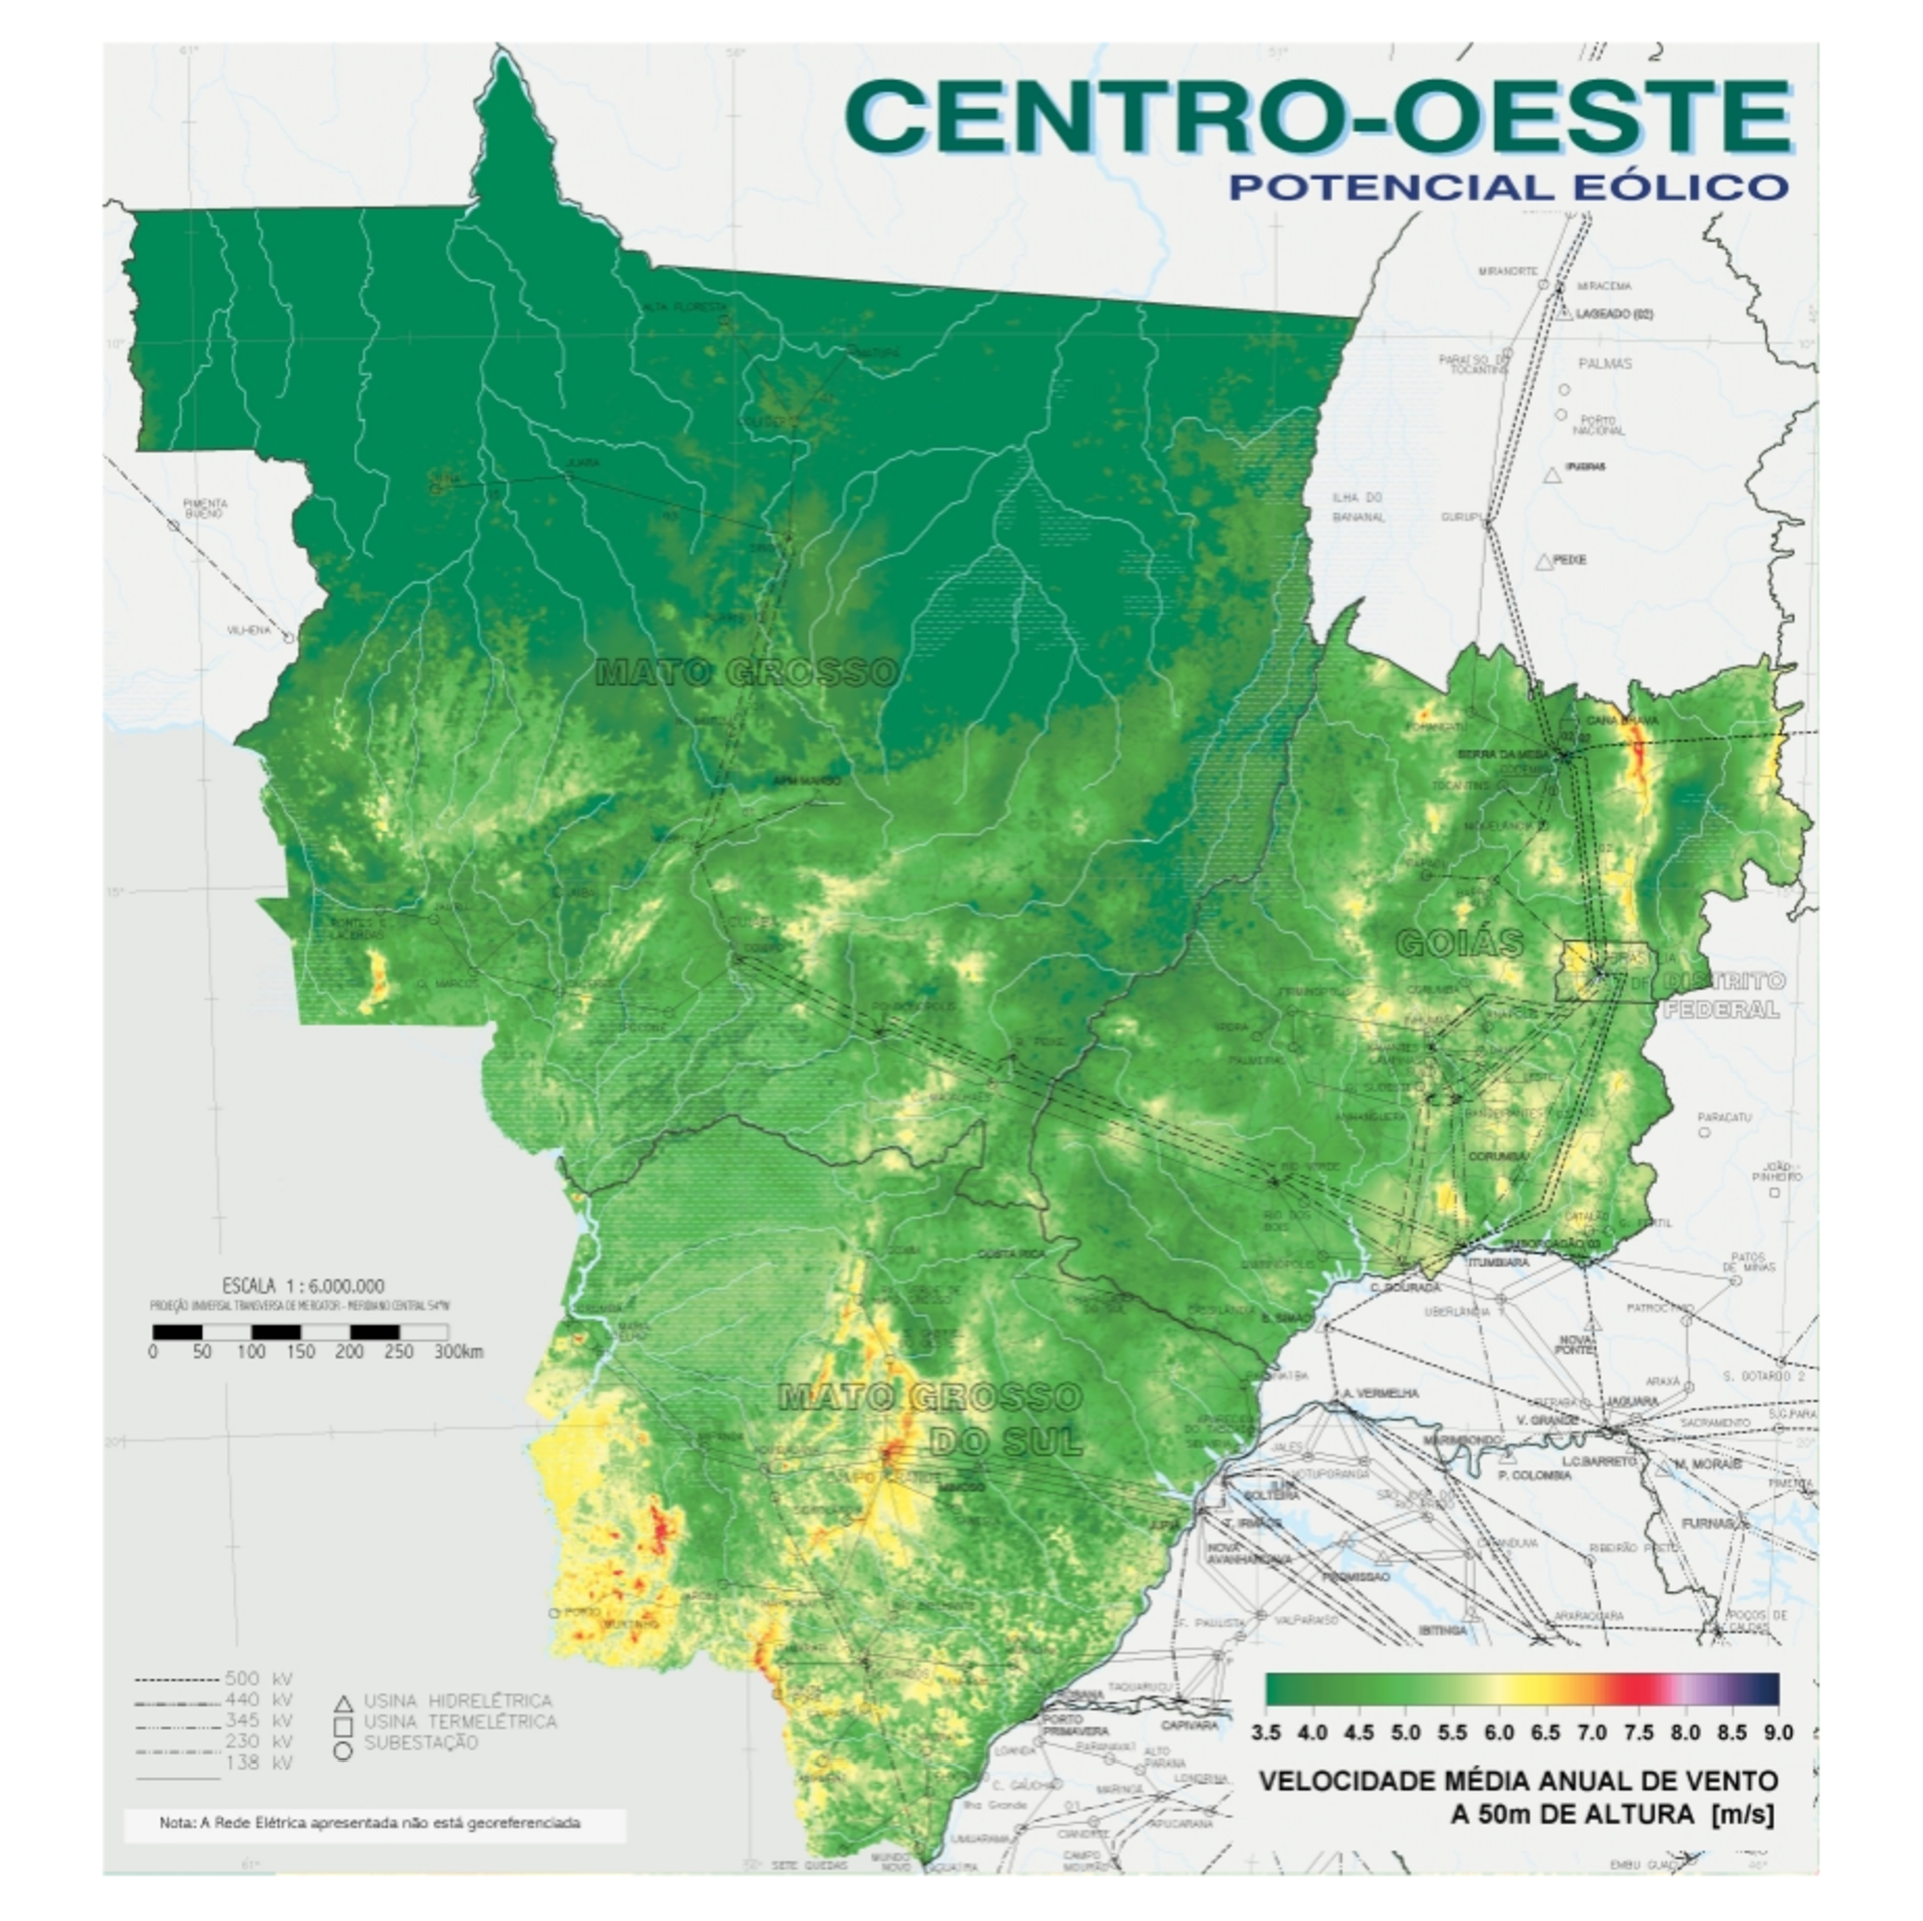
\includegraphics[width=.65\linewidth,keepaspectratio,angle=0]{figuras/potencial_centro_oeste.eps}
\caption{Potencial eólico na região Centro-Oeste.}
\label{potencial_centro_oeste}
\end{figure}


\begin{table}[H]
\centering
\begin{tabular}{|c|c|c|c|c|}
\hline 
\multirow{2}{*}{\textbf{Fontes}} & \textbf{Custo de implantação} & \multirow{2}{*}{\textbf{Eficiência}} & \textbf{Emissão de poluentes} & \multirow{2}{*}{\textbf{Manutenção}}\tabularnewline
 & \textbf{CESP/IMT {[}U\$/W{]}} &  & \textbf{{[}gCO2/kWh{]}} & \tabularnewline
\hline 
\hline 
Eólica & 1,00 & 42\% & 9,5 & Baixo custo\tabularnewline
\hline 
Solar & 5 à 10 & 15,4\% & 32 & Baixo custo\tabularnewline
\hline 
\end{tabular}
\caption{Comparativo entre solar e eólica}
\label{comparativo_solar_eolica}
\end{table}

A tabela \ref{comparativo_solar_eolica} mostra uma comparação entre as duas fontes que serão usadas no projeto da casa sustentável. A energia solar, a princípio, será mais cara, mas com o tempo o seu custo será pago. E depois o consumidor irá receber lucros com a sua implantação. A energia eólica já está com um preço de mercado para concorrer com as outras fontes. Desta forma, a utilização destas fontes é vantajosa para o empreendimento pois o consumidor não terá prejuízo com sua implantação.





































\newpage

	As fontes utilizadas na casa serão solar e eólica. Por serem de produção independente, privando a residência da dependência do uso da energia elétrica fornecida pela concessionária de abastecimento. Em análise aos fatores ambientais, essas fontes se tornam bastante produtivas e de ótima escolha, pois não geram transtornos para os habitantes da casa e minimizam custos com manutenção quando comparadas às outras fontes renováveis.

	Segundo dados encontrados no site da \cite{2013Aneel} (Agência Nacional de Energia Elétrica), no que diz respeito à Energia Eólica, a região centro-oeste tem o potencial eólico entre as classes 2 e 3, ou seja, está num setor onde a velocidade média do vento está entre 3,0 à 11,0 m/s. Sendo mais específico o Distrito Federal, e de acordo com o Atlas Eólico Brasileiro, possui uma velocidade média eólica cerca de 3,5 m/s. Já sob a análise dos dados informados pelo \cite{INMET} (Instituto Nacional de Meteorologia), a velocidade eólica permanece quase que constante por todos os períodos do ano. Com essas informações, torna-se importante a sua consideração da energia eólica como uma das fontes de energia que abastecerá a residência.

	Em termos de energia solar, a região central do Brasil recebe maior incidência de radiação solar durante as estações secas, particularmente entre os meses de julho a setembro, quando a precipitação é baixa e o número de dias com o céu claro é maior. Segundo dados retirados do ATLAS Solarimétrico do Brasil \cite{2000UFPE}, a localização onde se encontra o DF possui uma média anual de insolação diária entre 6-7h. Outro fator considerável são as variações de temperatura e mudanças de clima durante os períodos no decorrer do ano, que não ocorrem por longas temporadas, tornando o clima quente, ensolarado e seco predominante ao longo do ano.

\subsection{Dimensionamento}

	Para o dimensionamento e justificativa das fontes de energia, atribuiu-se que o consumo da residência seja de 500kWh/mês por motivos de segurança, já que o valor estimado na tabela \ref{consumo_eletrodomesticos} refere-se apenas ao consumo médio de equipamentos comuns.

\subsection{Energia Eólica -- Especificações técnicas}

	A média, de acordo com o Atlas Eólico Brasileiro, de Brasília é 3,5 m/s. Logo, a potência gerada por essa velocidade será baixa. A energia produzida pelo vento será destinada para abastecimento das baterias de reserva, que funcionarão caso acabe a energia devolvida pela concessionária da rede elétrica.

	No mercado mundial de aerogeradores são produzidos diversos modelos e com diferentes especificações técnicas que se adaptam melhor às necessidades de cada um. Os modelos são separados em duas categorias, sendo eles: aerogerador de eixo horizontal e de eixo vertical. Como a energia eólica será uma fonte secundária, escolheu-se dois exemplares (um de cada modelo) de potência baixa.

\newpage

\begin{table}[H]
\begin{tabular}{|c|c|c|}
\cline{2-3}
\multicolumn{1}{c|}{} & \multicolumn{2}{c|}{\textbf{Aerogerador}}\tabularnewline
\cline{2-3}
\multicolumn{1}{c|}{} & \textbf{Eixo Vertical}\parnote{Aeolos Wind Turbine 600[\si{\watt}]} & \textbf{Eixo Horizontal\parnote{Air 40}}\tabularnewline
\hline
Energia & 100kWh/mês - 5,8 m/s & 40kWh/mês - 5,8 m/s\tabularnewline
\hline
Velocidade de arranque & 1,5 m/s & 3,1 m/s\tabularnewline
\hline
Faixa de velocidade  & \multirow{2}{*}{1,5 - 40 m/s} & \multirow{2}{*}{3,1 - 22 m/s}\tabularnewline
de geração  &  & \tabularnewline
\hline
Ruído & < 45 dB & Silencioso\tabularnewline
\hline
Altura da torre & 1,6 metros & 10 metros\tabularnewline
\hline
Garantia & 5 anos & 5 anos\tabularnewline
\hline
Manutenção & Livre & Livre\tabularnewline
\hline
Vida útil & 20 anos & 20+ anos\tabularnewline
\hline
Local da compra & Reino Unido & Brasil\tabularnewline
\hline
Preço & R\$ 3.600,00\parnote{Preço diretamente convertido em reais com a cotação do dolar à R\$ 4,07 referente ao dia 01/11/2015}\parnote{Valor em tólar U\$ 849,00} & R\$ 5.499,00\tabularnewline
\hline
\end{tabular}
\parnotes
\caption{Quadro comparativo entre os modelos de aerogeradores}
\label{aerogeradores_modelos}
\end{table}

%http://www.windturbinestar.com/5kwv-v-aeolos-wind-turbine.html
%http://www.solar.coppe.ufrj.br/eolica/eol_txt.htm
%http://www.fahor.com.br/publicacoes/TFC/EngMec/2014/Eudes_Klockner_Matte.pdf

\subsection{Escolha do Aerogerador}

	A escolha do aerogerador de eixo horizontal se deve ao fato deste estar mais presente no mercado, com mais opções. Além do mais, a garantia é brasileira. Já o aerogerador de eixo vertical seria importado, aumentando os custos devido à alta do dólar e os impostos.

	O aerogerador a ser utilizado é o Air 40.

\begin{figure}[H]
  \begin{center}
	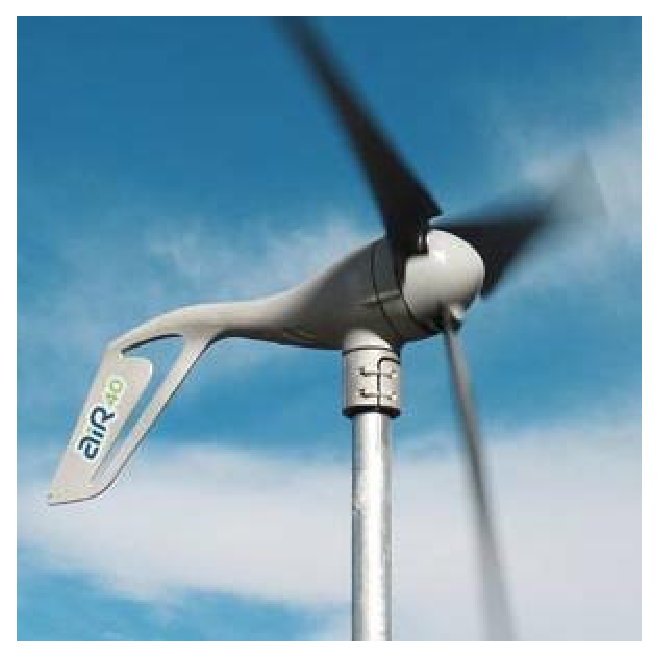
\includegraphics[keepaspectratio,scale=0.5]{figuras/air_40.eps}
	\caption{Aerogerador modelo Air 40}
  \end{center}
\end{figure}

%FONTE DA IMAGEM: https://www.energiapura.com/content/aerogerador-air-40

\subsection{Cuidados Específicos com o Aerogerador}

	Segundo informações do fabricante, apenas necessita-se manter as hélices limpas em períodos longos de seca.

\subsection{Localização de instalação do aerogerador}

	Quanto mais alto e direcionado para uma longa região livre de obstáculos aéreos, melhor. Pela sugestão do fabricante, e informações fornecidas pelo Prof. \cite{CORMANE} --, a melhor eficiência estará no aerogerador instalado acima de 10 metros do chão. Por ser pequeno, quando comparado aos aerogeradores de grande geração, o Air 40 pode ser instalado no teto da casa, com o suporte de uma haste para prolongar sua altura referente ao solo.

\subsection{Conexão dos painéis solares à rede}

	As placas fotovoltaicas serão on-grid, ou seja, conectadas à rede elétrica da concessionária. O consumo mensal estipulado é de 500kWh por mês. Logo, se trata de um sistema trifásico. Para que o sistema on-grid seja efetuado, é necessário a adesão obrigatória de uma taxa de disponibilidade da companhia energética, no qual de 100kWh por mês. Portanto, o sistema será dimensionado para 400kWh mensal [\cite{2013Aneel} -  Resolução Normativa ANEEL nº 482/2012].

\subsection{Dimensionamento da quantidade de painéis}

	Para determinar o número de placas solares, primeiro necessita-se conhecer a quantidade de energia consumida diariamente. Para isso basta fazer um cálculo simples onde se divide a energia mensal pelo número de dias. Sendo: energia consumida$\ = 400 \si{\kilo\watt\hour}/mês = 13,33 \si{\kilo\watt\hour}/dia$. Em seguida, precisa-se conhecer o índice solarimétrico médio por dia em Brasília \cite{2000UFPE}. Esse índice determina a quantidade de irradiação solar o local recebe por dia.

	Índice solarimétrico local de Brasília: $I_s\ =\ 5,13\ \si{\hour}/dia$

	Por fim, a potência das placas é definida a partir da razão entre a energia consumida pelo índice solarimétrico:$$P_p\ =\ 13333,33/I_s\ =\ 2600\ [\si{\watt}]$$

	Considerando uma eficiência de $0,85\%$, devido a perdas de geração e transmissão, $$P_t = 2600/0,85 = 3060 [\si{\watt}]$$

	Com a placa de potência de 255 W, pode-se obter a quantidade de painéis solares a partir da seguinte expressão: $N_{placas} = 3060/255 = 12$ placas no total

	Logo, serão necessárias 12 placas de $255 [\si{\watt}]$.

\subsection{Direção de instalação das placas para melhor geração de energia}

	A melhor direção para a instalação dos painéis é virada para a linha do Equador, no caso de Brasília está voltada para a direção Norte. Contudo, se houver um elevado nível de sombreamento nesta direção, sugere-se que os painéis então sejam colocados na face leste ou oeste do telhado da residência. Sabendo que, essa escolha poderá influenciar na quantidade de energia gerada. Vale enfatizar que, essas especificações visam a grosso modo o melhor aproveitamento da incidência solar na hora de instalar os módulos, pois há outras condições e variáveis que devem ser analisadas com mais cautela.

	No que se diz respeito à inclinação dos painéis, é importante que eles estejam a maior parte do período de insolação perpendiculares à direção de radiação solar, ou seja, igual ou o quão próximo possível à latitude da região. No caso, a melhor angulação para as placas deverá ser igual à 15,4$^o$.

\subsection{Manutenção dos módulo fotovoltaicos}

	O período de manutenção dos painéis não necessita de ser feita com uma determinada periodicidade, porém é preciso estar sempre atento aos sistemas de monitoramento e controle da energia produzida pelos painéis, sendo necessária a vistoria e limpeza em caso de queda na quantidade da potência.

	Já a limpeza dos módulos fotovoltaicos deve ser realizada na parte frontal, para que a eficiência não seja interferida, com o uso de um pano de microfibras e etanol sobre o vidro. Sendo esta realizada num período de 6 meses.

\subsection{Painel Estático vs Painel Móvel}

	Para fins comparativos, fez-se um levantamento de dados referentes à variação da angulação dos painéis solares de acordo com o horário e a direção de incidência solar. Comparando-se o modelo de painel solar fixo, onde sua angulação mantem-se constante por todo o dia, com um modelo de sistema onde os painéis solares teriam sua angulação ajustada conforme a mudança na direção da incidência dos raios solares, sistema similar ao que acontece com a planta Girassol. No entanto, concluiu-se que:

	“O ângulo de incidência solar tem um baixo grau de influência na geração fotovoltaica, ainda mais se levarmos em consideração que, na prática, ângulos de incidência elevados (superiores a 70$^o$) quase não acontecem, e se acontecem, apenas por curtos períodos de tempo (nascer e pôr-do-sol). A partir desta análise, e dos resultados obtidos até o momento, admite-se que um protótipo seguidor solar automatizado para microgeração solar não é viável financeiramente, pois se avalia que o ganho de tensão elé- trica (cerca de 11\% a pleno sol e em comparação a um ângulo de 70$^o$) não é suficiente para alimentar um motor que fique rotacionando o painel ao longo do dia.” \cite{2011PUCAMP}

%Fonte: https://www.puc-campinas.edu.br/websist/portal/ceatec/hidro/subprojetos/arquivos/Avaliacao-influencia-angulo-incidencia.pdf

\section{Tecnologia de Armazenamento}

\subsection{Definição}

	As tecnologias de armazenamento tem como intuito “guardar” a energia gerada pelos painéis solares e o aerogerador e transformá-la em eletricidade, e o excedente ser depositado em algum “lugar” ou alocado. Podendo ser elas em forma de baterias, acumuladores de energia, ou sistemas inteligentes interligados à rede elétrica.

\subsection{Tecnologias Utilizadas}

	Para o armazenamento das energias geradas pelos painéis solares e pelo aerogerador, têm-se duas propostas, sendo uma o uso de baterias residenciais e a outra consiste num sistema grid-tie em que serve para "jogar" na rede elétrica a energia excedente. Como o sistema grid-tie funciona apenas para fazer uma espécie de troca de energia com a companhia de energia elétrica, isso não impede que a casa sofra quedas de energias e apagões. Por ser a fonte primária de geração de energia e mais eficientes, os painéis solares serão ligados ao sistema com a rede. Já a energia produzida pelo aerogerador servirá para recarregar e armazenar em baterias. O uso das baterias tem como premissa a continuidade do fornecimento de eletricidade na casa, mesmo em apagões.

	As tecnologias de armazenamento mais comuns e que se adequam às necessidades da casa são: o uso de baterias residenciais e um sistema grid tie.

\subsection{Como funciona cada tecnologia adotada}

	Sistemas Grid-Tie, se refere a um dispositivo eletrônico que permite aos usuários de energia solar ou eólica interligar seus sistemas com a rede da concessionária e injetar na rede o excedente de energia produzido pelos sistemas (fotovoltaico ou eólico). Esse sistema gerará um custo inicial alto, porém a sua manutenção é demorada e o retorno quanto a economia e o custo da energia elétrica oferecida pelas concessionárias compensa em pouco tempo de uso.

	Se trata de um dispositivo eletrônico que será conectado aos painéis solares, interligando seus sistemas com a rede da concessionária e injetando na rede o excedente de energia produzido. Funcionando da seguinte forma, quando proprietário do sistema produzir mais energia do que consome, a energia produzida fará com que o medidor “gire para trás”. Quando produzir menos do que consome, o medidor deverá “girar mais devagar”. Vale observar que o medidor deve ser apropriado para contabilizar o fluxo de energia nos dois sentidos.

	Já as baterias residenciais servirão para armazenar parte da energia produzida e utilizadas quando houver picos de energia quanto à energia retornada pela concessionária, ou afim de economia referente às tarifas. Atualmente, têm-se as baterias automotivas que são mais encontradas para fazer esse tipo de armazenamento, porém para isso deve-se fazer algumas adaptações e associar um grande número de baterias para que elas consigam reabastecer de forma significante a eletricidade da casa. Em contrapartida, recentemente a empresa especializada em automóveis elétricos \cite{TESLA} apresentou no início do ano (2015) baterias feitas para o uso residencial, a PowerWall. Tais baterias tem como proposta melhorar a autonomia da casa em relação à dependência da companhia energética local. Com duas capacidades, a \cite{TESLA} apresenta o modelo de bateria residencial com capacidade de armazenamento de 7kWh e 10kWh, custando respectivamente U\$ 3000 e U\$ 3500. Já disponíveis para compra no site da empresa. As baterias podem ser associadas em série e afixadas a qualquer lugar da casa \cite{TESLA}.

\begin{figure}[H]
  \begin{center}
	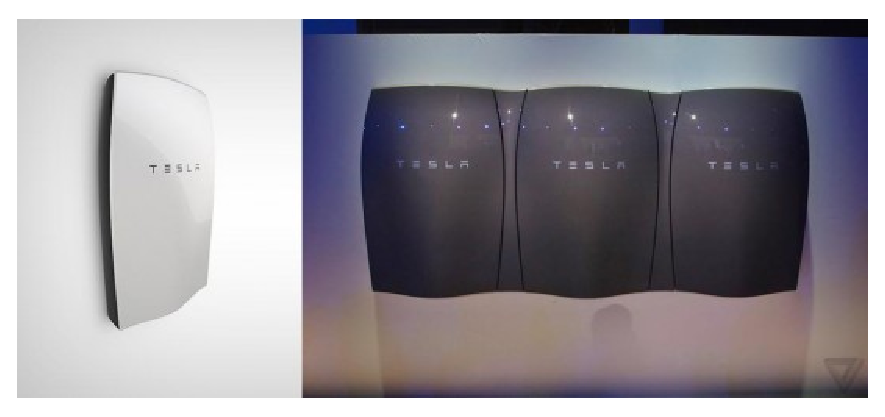
\includegraphics[keepaspectratio,scale=1]{figuras/powerwall.eps}
	\caption{Powerwall}
  \end{center}
\end{figure}
%FONTE: http://www.teslamotors.com/powerwall?

\subsection{Quantidade de baterias necessárias}

	Para o projeto da casa, necessita-se de no máximo 5 baterias, no qual essas já teriam capacidade de alimentar a residência em suas necessidades básicas (como cozinha, iluminação e equipamentos de monitoramento e de segurança), por vários dias no caso de apagão.

\subsection{Local de instalação}

\textbf{a. Área ocupada:}

	O seu dimensionamento é de 130cmx68cmx18cm para cada uma, e funcionando na faixa de temperatura -20°C a 43°C \cite{TESLA}
%FONTE: http://www.teslamotors.com/powerwall?

\subsection{Especificações e garantia das baterias}

	Essas baterias apresentam uma conexão com a internet, onde é possível o monitoramento da energia armazenada e quanto está sendo gasta. Tais baterias quando carregadas e descarregadas entre 20\% e 80\% do seu total de armazenamento, com vida útil de 1500 ciclos, durariam por anos, tendo uma garantia de 10 anos pela empresa \cite{TESLA}.
%FONTE: http://www.teslamotors.com/powerwall?

\subsection{Especificações do Sistema Grid-Tie}

	Para os painéis solares na casa, serão 12 placas ao todo, tendo duas ligações em série de 6 placas cada. Para esse sistema, tem-se duas opções de instalação dos inversores grid-tie, a modular e a central.

	\textsc{central} - Recebe energia de vários painéis solares, ligados em série e paralelo, estabilizando com um único otimizador MPPT e fazendo sua função de inversor DC/AC. Há um ganho de custo por utilizar menor número de inversores, porém há menor flexibilidade de projeto e manutenção.

	\textsc{modular} - Cada inversor recebe uma série ou string e vários inversores são utilizados em paralelo, cada um com seu otimizador MPPT. Essa configuração permite maior flexibilidade, como diferentes orientações para cada string. Além disso, eventuais perdas com defeitos, sujeiras, sombreamentos, etc. são minimizados pois cada série funciona separadamente.

	Devido à quantidade dos painéis solares, e mantendo-se a manutenção e os devidos cuidados para sempre manter a eficiência em alta com os painéis, o opção pelo sistema central já é capaz de satisfazer as necessidades da família e tendo uma melhor relação entre custo-benefício.

\subsection{Manutenção}

	Tal produto dispensa manutenção desde que suas condições de operação sejam seguidas, tais como estar em ambientes com temperaturas entre $-25^oC$ e $+50^oC$, entre outras especificações técnicas. O produto possui garantia de 5 anos e vida útil acima de 10 anos.

%FONTE: http://www.neosolar.com.br/loja/kit-gerador-solar-fotovoltaico-fronius-300-kwp-420-kwh.html

\subsection{Controle da quantidade gerada e consumida}

	O controle pode ser feito diretamente olhando ao quadro de energia, ou por meio de recebimento de dados, já que os inversores presentes atualmente no mercado possuem sistema de monitoramento integrado à conexão WLAN.

%FONTE: http://www.neosolar.com.br/loja/kit-gerador-solar-fotovoltaico-fronius-300-kwp-420-kwh.html

\section{Reaproveitamento da água}

\subsection{Consumo de água médio pela família}

	De acordo com a Organização das Nações Unidas, cada pessoa necessita de 3,3 mil litros de água por mês (cerca de 110 litros de água por dia para atender as necessidades de consumo e higiene). No entanto, no Brasil, o consumo por pessoa pode chegar a mais de 200 litros/dia. Atualmente, cada habitante do DF consome, em média, 190 litros diários, de acordo com a Companhia de Saneamento Ambiental do Distrito Federal \cite{CAESB}.

	Em Brasília o consumo médio por habitante é de 190 litros de água/dia, o que resulta em um consumo mensal médio de $6\si{\meter}^3$ por habitante. Para a casa com 4 habitantes, o consumo mensal médio será de $24\si{\meter}^3$.

\subsection{Reutilizar a água - Justificativa}

	Por se tratar de um bem natural que está cada vez mais raro e caro, reutilizar a água é de fundamental importância para o meio ambiente e também para a economia das empresas, cidadãos e governos. Evitar o desperdício é a chave para a preservação.

\subsection{Água reaproveitada}

	Será reaproveitada a água cinza que consiste em qualquer água residual, a partir de processos domésticos como lavar louça, roupa e tomar banho. A água cinza corresponde de 50\% a 80\% de esgoto residencial e a água da chuva que será armazenada e desse armazenamento resultará em um aproveitamento de 100\%.

	Já a água da chuva pode muito bem ser utilizada em descargas sanitárias, irrigação de jardins, limpeza de calçada, pátios, paredes, veículos, em espelhos e fontes d’água, sistemas de resfriamentos, entre outros, economizando assim a água tratada, que poderá ser usada apenas para fins mais nobres.

\subsection{Finalidade da água não aproveitada}

	A água não aproveitada ou também chamada de água negra, geralmente água do vaso sanitário será descartada na rede de esgoto.

	O esgoto produzido pela residência será despejado na rede, pois com relação ao índice de atendimento à população, segundo dados do censo demográfico 2010 realizado pelo \cite{IBGE}, 88,9\% das residências urbanas possuem saneamento adequado e 10,9\% semi-adequado. Esses dados sugerem que o Distrito Federal possui o maior índice de cobertura de saneamento no Brasil, que acaba mostrando que é explicitamente mais viável utilizar a rede pública.

	A empresa responsável pelo tratamento é a \cite{CAESB}, que possui um nível de tratamento terciário do esgoto, enquanto outras empresas utilizam apenas o tratamento secundário, que é um dos motivos que diferencia as ETE's do DF das demais. O tratamento a nível primário são sedimentados os sólidos em suspensão que vão se acumulando no fundo do decantador, formando o lodo primário que depois é retirado para dar continuidade ao processo. Em seguida, no tratamento a nível secundário, os microrganismos irão se alimentar da matéria orgânica, convertendo-a em gás carbônico e água. E por final, no tratamento a nível terciário são removidos poluentes específicos como micronutrientes (fósforo e nitrogênio) o que garante a qualidade ainda maior do tratamento.

	Outra característica importante na escolha do tratamento de esgoto da rede pública é que ao analisarmos o esgotamento sanitário no DF, os lodos de esgoto, em geral, possuem concentrações de substâncias químicas dentro dos limites estabelecidos pela legislação, e desse modo a \cite{CAESB} incentiva a destinação ambientalmente equilibrada desses lodos por meio de sua incorporação ao solo agricultável, isto é, por meio da reciclagem dos seus nutrientes e matéria orgânica em atividades de agricultura, de silvicultura ou de recuperação de áreas mineradas.

\subsection{Processo de captação da água}

	No processo de captação da chuva, é necessário ter na construção um sistema de captação e armazenamento dessa água. O princípio desses sistemas é simples: a água é captada antes que entre em contato com o solo ou local de trânsito de pessoas, animais e veículos, evitando assim contaminação, através de telhados e calhas que direcionam a água para um filtro autolimpante que irá retirar os resíduos e levá-la diretamente para cisternas \cite{EMBRAPA}.

%FONTE: http://www.alice.cnptia.embrapa.br/alice/bitstream/doc/129165/1/OPB420.pdf

\subsection{Processo de tratamento da água cinza}

	Referente ao processo de tratamento da água cinza seguiremos o modelo aplicado experimentalmente na \cite{UFES}.

	Primeiramente, um reservatório receberá essa água, geralmente composto por caixas de retenção. Em seguida o efluente dessa água se direciona a um elevatória de água cinza bruta, para então seguir para um reator anaeróbico (sem oxigênio), onde a matéria orgânica é estabilizada. Depois a água passa por um filtro biológico aerado submerso que visa eliminar o odor de substância químicas. Então vai para um decantador secundário para seguir ao filtro terciário. Por fim passa pela elevatória de água cinza tratada para chegar no reservatório superior de água de reuso.

\subsection{Dimensionamento e local da instalação da cisterna}

A cisterna será implementada no quintal da casa ou subsolo com capacidade de 16 mil litros de água, é necessário um acompanhamento periódico da cisterna, assim como o centro de tratamento da água cinza.

\subsection{Manutenção necessária}

	As áreas de captação têm que ser limpas; as calhas têm que ser mantidas em boas condições; a água não pode ser retirada com baldes, que foram colocados no chão, para evitar contaminação.

	Desta maneira, uma instalação de captação de água de chuva pode fornecer água potável de ótima qualidade, requer um investimento único, não apresenta custos de manutenção, não tem partes móveis, tanto que a manutenção pode ser feito até por crianças, e ainda por cima é a solução ecologicamente mais correta (ECOCASA).
%FONTE: http://www.ecocasa.com.br/cisternas.asp

\section{Reutilização do lixo doméstico}

\subsection{Lixo produzido}

	No Brasil, são coletados aproximadamente 173.583 de toneladas de lixo por dias de acordo com o Panorama de resíduos sólidos no Brasil realizado pela \cite{ABRELPE} em 2010. Sendo que 99.919t/d (57,6\%) são destinados a aterros sanitários, 42.231 (24,3\%) vão para aterros controlados que, segundo a \cite{NBR8849:1985}, é uma técnica de disposição de resíduos sólidos urbanos no solo, que consiste na cobertura desses resíduos com uma camada de material afim de confiná-lo. E o restante de 31.433 t/dia (18,1\%) é distribuído em lixões.

	No Distrito Federal, são coletados diariamente 3.951t/dia de lixo, sendo 1,596kg produzido por cada habitante diariamente, o que torna Brasília a maior produtora de lixo por habitante do Brasil e a maior parte deste, é destinado a aterros controlados, com base em informações da \cite{ABRELPE}. Tomando como base a média regional, a quantidade de moradores da residência e possíveis visitas de pessoas na mesma, a quantidade de resíduos sólidos produzidos diariamente na casa, sendo eles recicláveis ou orgânicos, é de 7,980 kg/hab/dia

\subsection{Lixo destinado ao serviço de limpeza urbana}

	O Distrito Federal tem os serviços de saneamento prestados pela Companhia de Saneamento Ambiental do DF\cite{CAESB} (água e esgoto), pela \cite{Novacap} (drenagem urbana) e pelo \cite{SLU} (limpeza urbana e manejo de resíduos sólidos).

	Com base no Relatório de Diagnósticos de Resíduos Sólidos realizado pelo \cite{SLU} do DF, a quantidade de lixo coletado seletivamente pelo \cite{SLU}, chega a 9,88\% em toda a região, mas considerando rejeitos, apenas 2\% desse total foram encaminhados à reciclagem. Do total de lixo coletado no Jardim Botânico, cerca de 60\% dele faz parte da coleta seletiva.

	De acordo com a população do Distrito Federal e a quantidade de lixo coletado, é possível estimar que cerca de 60\% do lixo sólido gerado pela residência é seco e será destinado a coleta seletiva para reciclagem desses materiais. Pois no Jardim Botânico a coleta realizada pelo \cite{SLU} é realmente efetiva

\subsection{Detalhamento do processo de separação do lixo}

	A reciclagem reduz o impacto sobre o meio ambiente, gera economia de água e luz. Diminui as retiradas de matéria-prima da natureza e a disposição inadequada do lixo. Para o processo de separação do lixo residencial, será utilizada a prática dos 3 R's que é: reduzir, reciclar e reutilizar.

	O processo de separação dos resíduos sólidos da residência será feito manualmente pelos integrantes da família. Primeiramente, é necessário que a pessoa que faça a separação conheça e saiba diferenciar o lixo reciclável (papel, jornais, garrafas plásticas, recipientes de limpeza, latinhas de alumínio, embalagens e produtos eletroeletrônicos e entre outros) do lixo orgânico (cascas de frutas e legumes, sobras de alimento).

	Após a identificação de cada tipo de material, é necessário que o lixo reciclável seja limpo, seco e armazenado separadamente do lixo orgânico, para que possa ser entregue a coleta seletiva da região feita pelo \cite{SLU}. Já o lixo orgânico será separado manualmente para a utilização nas composteiras.

\subsection{Detalhamento do processo de reutilização do lixo orgânico}

	Visando as necessidades de se descartar o lixo orgânico corretamente, a residência terá uma composteira, que é basicamente um processo de decomposição e de reciclagem de matéria orgânica contida em restos de origem animal ou vegetal, formando um composto rico em substâncias húmicas e nutrientes que podem ser como adubo na manutenção do jardim.

	Na escolha do modelo mais adequado para a residência, foi escolhido uma composteira automática que é movida a energia elétrica e acaba se tornando um método mais prático e simples de se fazer a compostagem. As vantagens na utilização desse tipo de composteira ao invés da convencional, é pelo fato de que ela pode ser instalada em praticamente qualquer espaço da casa, não requer muito conhecimento para manuseio do aparelho, não traz problemas com odores. Outro fator relevante é o tempo que ela leva para compostar o alimento, que é de 24h ao contrário das convencionais que podem levar até 60 dias.

	A composteira elétrica funciona diferentemente da convencional que possui minhocas no seu processo. Nela se faz o uso de poderosos microrganismos patenteados capazes de se multiplicarem em altas temperaturas, acidez, salinidade e que possuem uma alta longevidade o que torna a manutenção sem custos adicionais.

\subsection{Local e dimensionamento da composteira}

	O modelo de composteira para utilização é o Decomposer 2, que possui 40x40cm de comprimento e 78cm de altura, pesa 21kg e consome cerca de 60-80kWh/mês, e tem capacidade diária de compostagem de aproximadamente 5,5kg de resíduos orgânicos o que é adequado para uma família de 4 pessoas.  A máquina possui três funções que é a de agitação, calor e fluxo de ar, o que torna o processo muito simples.

	A composteira será colocada dentro da cozinha, e para ser utilizada, basta apenas que a pessoa despeje o lixo orgânico dentro da composteira e ligue o aparelho. Após 24h o adubo pode ser retirado e utilizado para manutenção do jardim da residência.

%Fonte: http://www.ecycle.eco.br/index.php/composteiras/composteira-decomposer-2.html

%REFERENCIAS
%GOLDEMBERG, José; LUCON, Oswaldo. Energias Renováveis: Um futuro sustentável. REVISTA USP – 2007. Disponível em: www.revistas.usp.br/revusp/article/download/13564/15382
